% INTRODUCCIÓN

\cleardoublepage

\chapter{Introducción}
\label{chapter-introduccion}

\section{Procesamiento Natural del Lenguaje}
\label{section-procesamiento-natural-lenguaje}

Los últimos años hemos sido testigos del auge de la inteligencia artificial y del impacto que esta ha generado en distintos aspectos de nuestras vidas, convirtiéndose en una tecnología que ha cambiado la forma en la que interactuamos y vivimos. Hemos presenciado sorprendentes avances de la inteligencia artificial en distintos ámbitos y la evolución que ha tenido en la resolución de muchas tareas específicas, logrando en varias de ellas superar las capacidades cognitivas propias de los seres humanos. 

El \acrlong{acr_nlp} (\acrshort{acr_nlp}, por sus siglas en inglés) es una rama de la inteligencia artificial que habilita a las computadoras a comprender, entender y procesar el lenguaje humano. El \acrshort{acr_nlp} provee de un conjunto de técnicas y metodologías para analizar, interpretar y darle significado al lenguaje y de este modo, poder generar conocimiento a partir de este. 

El \acrshort{acr_nlp} se ha convertido en una de las tareas más complejas a resolver en la búsqueda de recrear las capacidades cognitivas propias de los seres humanos a través de las máquinas. Y es que, sin lugar a duda, el lenguaje humano es un proceso bastante complejo que ha sido el resultado de la propia evolución a lo largo de miles de años y sustentado por un motor biológico con más de cien mil millones de neuronas que interactúan entre sí. 

Para hacerlo aún más complejo, nuestro lenguaje está lleno de ambigüedades, de palabras con distintas acepciones, giros y diversos significados según el contexto y además elementos que aún son de difícil comprensión como la ironía o el sarcasmo. Esto hace que el procesamiento de lenguaje natural haya sido una de las tareas más difíciles de dominar en el mundo de la inteligencia artificial.
\medskip

\section{El aprendizaje automático y el NLP}
\label{section-antes-de-las-redes-neuronales}

En este camino del entendimiento y comprensión del lenguaje humano por las maquinas, se han explorado distintas soluciones desde algoritmos o arquitecturas basadas en reglas donde se intenta modelar instrucción a instrucción y a través de reglas complejas, hasta soluciones donde dejamos que algoritmos puedan inferir estas reglas a través del \acrlong{acr_ml} (\acrshort{acr_ml}, por sus siglas en inglés). 

El \textit{machine learning} a pesar de ser una disciplina con muchos años de investigación, ha ganado una relevancia considerable en los últimos años debido al aumento cada vez mayor de la capacidad de cómputo y con ello la habilidad de poder procesar grandes cantidades de datos. Esto ha posibilitado el desarrollo acelerado del \textit{machine learning} y los modelos de \acrlong{acr_dl} (\acrshort{acr_dl}, por sus siglas en inglés). Las redes neuronales artificiales ocupan una posición muy prometedora en el área del \textit{machine learning} y han transformado la forma en que se desarrollan las aplicaciones de \acrshort{acr_nlp}. 

Para este tipo de problemas donde el dato de entrada es un texto de naturaleza secuencial, se han explorado distintas arquitecturas que van desde las redes neuronales recurrentes (ver sección \ref{section-rnn}), pasando por las redes \textit{long short-term memory} (ver sección \ref{section-lstm}), hasta las poderosas redes basadas en la novedosa arquitectura de \Gls{gls_transformer}, concepto sobre el que se profundizará en la sección \ref{subsection-atencion-transformer}.

\subsection{Redes Neuronales Recurrentes (RNN)}
\label{section-rnn}

Las \acrlong{acr_rnn} (\acrshort{acr_rnn}, por sus siglas en inglés), son un tipo de redes que tienen un excelente desempeño para el análisis de datos que tienen una naturaleza secuencial, es decir, datos donde el orden tiene importancia relevante. Es por ello, que generalmente es empleada en los problemas de procesamiento de audio, vídeo o texto. La idea es que los datos de entrada tengan una cierta secuencia adjunta como en los textos donde la secuencia de palabras genera un contexto que agrega significado a la oración. 

Como es explicado por \cite{torres2019deep}, las redes neuronales recurrentes fueron concebidas en la década de 1980. Pero estas redes fueron en un principio difíciles de entrenar por sus requerimientos en computación y no es solo hasta estos últimos años, en los que se generaron grandes avances en temas de capacidades de cómputo y procesamiento, que este tipo de redes se han hecho más accesibles y se ha popularizado su uso.

El aspecto más importante de las \acrshort{acr_rnn} es que funcionan en bucles, los datos fluyen circularmente, en consecuencia aprenden no solo la entrada del estado actual sino también la entrada anterior. Se dice entonces que este tipo de red incorpora la retroalimentación lo que consigue crear un concepto de temporalidad, permitiendo a la red tener ``memoria''.

En un modelo de red típico, la función de activación solo actúa en una dirección, hacia delante, desde la capa de entrada hacia la capa de salida, es decir, que no recuerdan valores previos. Una red \acrshort{acr_rnn} es parecida, pero incluye conexiones que apuntan ``hacia atrás'', una especie de retroalimentaciones entre las neuronas dentro de las capas.

Siguiendo esta misma idea, una capa de neuronas recurrentes se puede implementar de tal manera que, en cada instante de tiempo, cada neurona recibe dos entradas, la entrada correspondiente de la capa anterior y a su vez la salida del instante anterior de la misma capa, como es mostrado en la figura ~\ref{fig-intro-arq-rnn}.

\begin{figure}[ht!]
    \centering
    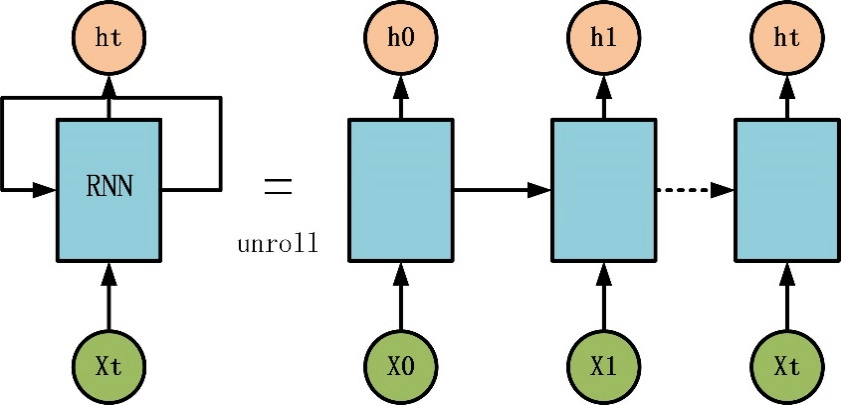
\includegraphics[scale=0.3]{figuras/intro-arq-rnn.png}
    % \caption[Así aparece el rótulo en el índice]{Así aparece el rótulo en el texto.}
    \caption[Arquitectura de red neuronal recurrente (RNN)]{\textbf{Arquitectura típica de una red neuronal recurrente, donde podemos observar la secuencia y la relación de cada celda con los estados anteriores. Fuente: \citep{articleFang2020LSTM}}}
    \label{fig-intro-arq-rnn}
\end{figure}

Precisamente esta ``memoria interna'' es lo que hace a este tipo de redes muy adecuadas para problemas de aprendizaje automático que involucran datos secuenciales. Gracias a su ``memoria interna'', las \acrshort{acr_rnn}s pueden recordar información relevante sobre la entrada que recibieron, lo que les permite ser más precisas en la predicción de lo que vendrá después, manteniendo información de contexto a diferencia de los otros tipos de redes que no pueden recordar acerca de lo que ha sucedido en el pasado, excepto lo reflejado en su entrenamiento a través de sus pesos.

Dos conceptos importantes que afectan a las \acrshort{acr_rnn} son los gradientes explosivos (\textit{exploding gradient}, en inglés) y el desvanecimiento del gradiente (\textit{vanishing gradients}, en inglés), aunque ambos efectos son propios en general de cualquier tipo de red muy grande en números de parámetros, sea o no sea recurrente. 

Estos conceptos son bien descritos por \cite{torres2019deep}, recordando que el gradiente indica el cambio a realizar en todos los pesos con respecto al cambio en el error, en tal sentido, hablamos de ``gradientes explosivos'' cuando el algoritmo asigna una importancia exageradamente alta a los pesos, sin mucha razón y esto genera un problema en el entrenamiento y hablamos de ``gradientes desaparecidos'' cuando los valores de un gradiente son demasiado pequeños y el modelo deja de aprender o requiere demasiado tiempo debido a ello. 

\subsection{Redes Long Short-Term Memory (LSTM)}
\label{section-lstm}
Como se describe en la sección anterior, las redes neuronales recurrentes convencionales presentan problemas en su entrenamiento debido a que los gradientes retropropagados tienden a crecer enormemente o a desvanecerse con el tiempo debido a que el gradiente depende no solo del error presente sino también los errores pasados. La acumulación de errores provoca dificultades para memorizar dependencias a largo plazo.

Las \acrlong{acr_lstm} (\acrshort{acr_lstm}, por sus siglas en inglés), son una extensión de las redes neuronales recurrentes, que como indica \cite{thomas2020natural}, fue propuesta por Sepp Hochreiter y Jürgen Schmidhuber en 1997 para abordar el problema de los gradientes explosivos y desaparecidos. Este tipo de redes básicamente amplían su memoria para aprender de experiencias importantes que han sido analizadas hace mucho tiempo en la secuencia. Las \acrshort{acr_lstm} permiten a las \acrshort{acr_rnn}s recordar sus entradas durante un largo período de tiempo. Esto se debe a que \acrshort{acr_lstm} contiene su información en la memoria, que puede considerarse similar a la memoria de un ordenador, en el sentido que una neurona de una \acrshort{acr_lstm} puede leer, escribir y borrar información de su memoria.

En una neurona \acrshort{acr_lstm} hay tres puertas que controlan el modo en que la información fluye dentro o fuera de la unidad: puerta de entrada (\textit{input gate}), puerta de olvidar (\textit{forget gate}) y puerta de salida (\textit{output gate}), como muestra la figura ~\ref{fig-intro-arq-lstm}. Estas puertas determinan si se permite o no una nueva entrada, se elimina la información porque no es importante o se deja que afecte a la salida en el paso de tiempo actual.

\begin{figure}[ht!]
    \centering
    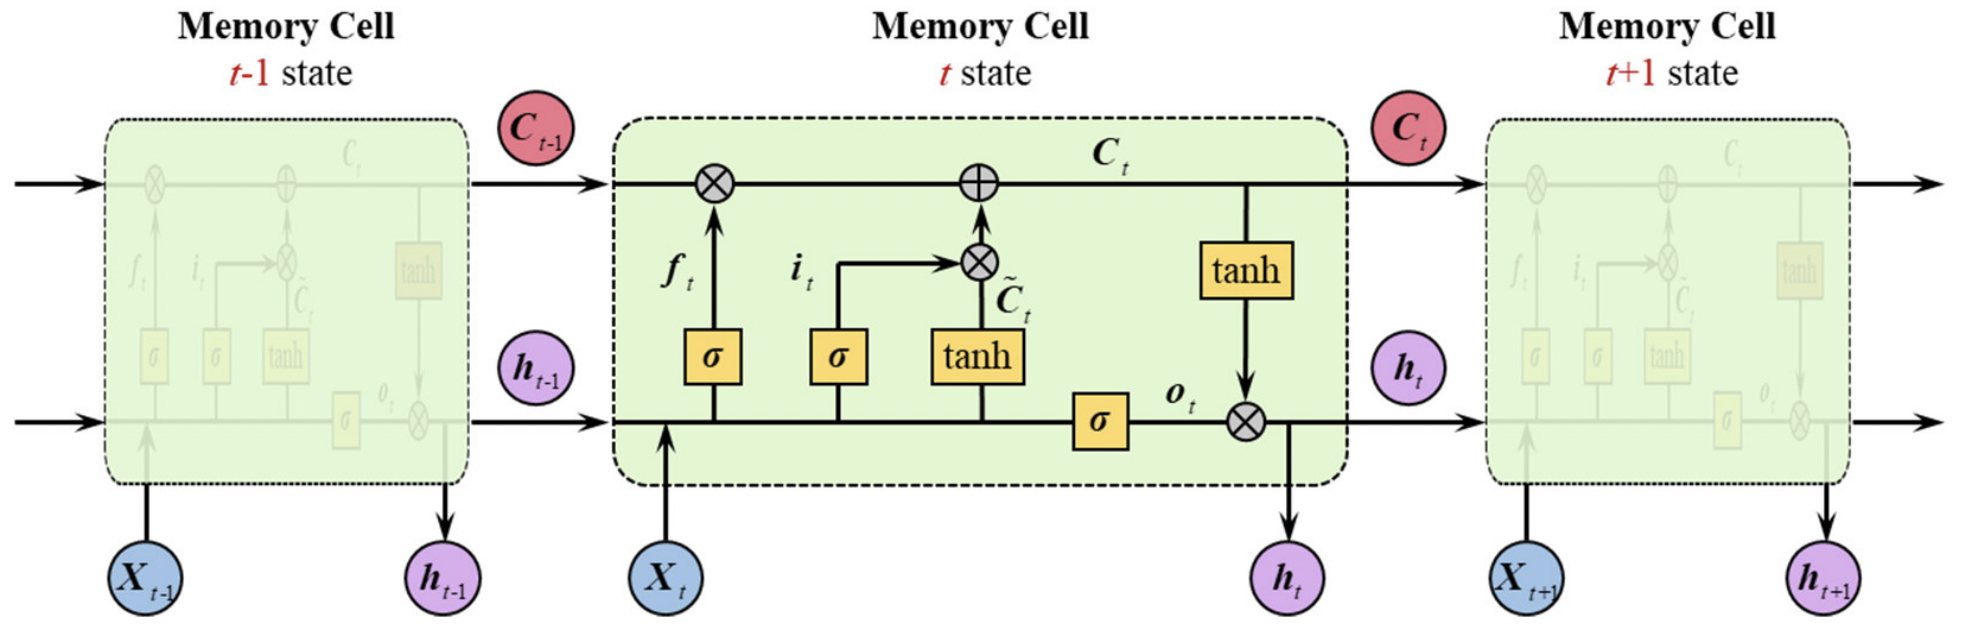
\includegraphics[scale=0.4]{figuras/intro-arq-lstm.png}
    % \caption[Así aparece el rótulo en el índice]{Así aparece el rótulo en el texto.}
    \caption[Arquitectura de red Long Short-Term Memory (LSTM)]{\textbf{Mirada interna a una celda de memoria en una red de tipo Long Short-Term Memory (LSTM). En la imagen se pueden observar los tres tipos de puertas presentes en la neurona. Fuente: \citep{LSTM_Olah_2015}}}
    \label{fig-intro-arq-lstm}
\end{figure}

\section{Bidirectional Encoder Representations from Transformer}
\label{section-bert}

\textbf{BERT} siglas para \textit{\textbf{B}idirectional \textbf{E}ncoder \textbf{R}epresentations from \textbf{T}ransformers} es un poderoso modelo de lenguaje publicado por investigadores de Google en octubre de 2018 que usa dos etapas, el preentrenamiento y el ajuste fino (\textit{fine-tunning}, en inglés), para crear modelos muy eficientes capaces de resolver  una amplia gama de tareas relacionadas al procesamiento de lenguaje natural \citep{https://doi.org/10.48550/arxiv.1810.04805}.

Desde su aparición BERT ha causado revuelo en la comunidad del \textit{machine learning} producto de su característica arquitectura que permite que el mismo modelo preentrenado se pueda ajustar para resolver una variedad de tareas finales que pueden no ser similares a las tareas para las que en un principio se entrenó y obtener resultados similares a los que definen el estado del arte para estas tareas en el campo del \acrshort{acr_nlp} (ver figura \ref{fig-intro-bert-transfer}), lo que define el objetivo principal de este trabajo (ver sección \ref{section-objetivo-general}). Los modelos como BERT y sus similares han superado varios puntos de referencia importantes en tareas de procesamiento de lenguaje natural. 

\begin{figure}[ht!]
    \centering
    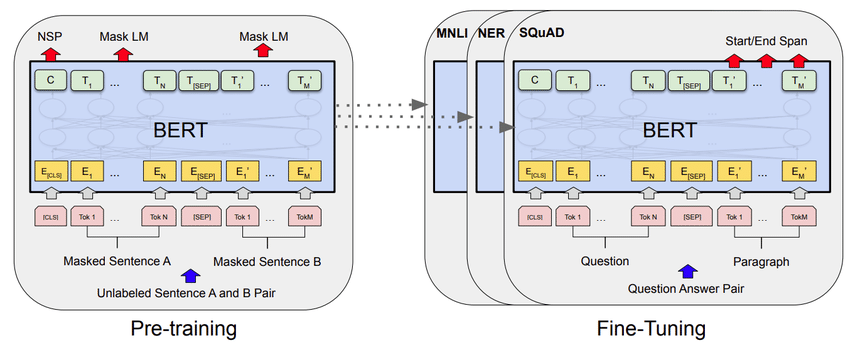
\includegraphics[scale=0.5]{figuras/intro-bert-transfer.png}
    % \caption[Así aparece el rótulo en el índice]{Así aparece el rótulo en el texto.}
    \caption[BERT - Transfer Learning]{\textbf{Procedimientos generales de preentrenamiento y fine-tunning en BERT. BERT utiliza la misma arquitecturas tanto en el preentrenamiento como en el fine-tuning. Los parámetros del modelo preentrenado se utilizan para inicializar modelos para resolver otras tareas. Fuente: \citep{https://doi.org/10.48550/arxiv.1810.04805}}}
    \label{fig-intro-bert-transfer}
\end{figure}

\subsection{Mecanismos de Atención y Transformer}
\label{subsection-atencion-transformer}

La base de BERT es el modelo \Gls{gls_transformer}, un tipo de red neuronal propuesta recientemente, basada en mecanismos de atención, que acepta como entrada datos secuenciales (por ejemplo, una secuencia de palabras) y produce algún resultado (por ejemplo, la predicción de sentimientos). A diferencia de las redes recurrentes tradicionales, como las LSTM, que procesan cada elemento de secuencia uno a la vez, con \Gls{gls_transformer} se procesan todos los elementos simultáneamente (autoatención) formando conexiones directas entre todos los elementos. Esto no solo permite una mayor paralelización, sino que también da como resultado una mayor precisión en una variedad de tareas, lo que le ha permitido impulsar importantes avances en el procesamiento del lenguaje natural.

\begin{figure}[ht!]
    \centering
    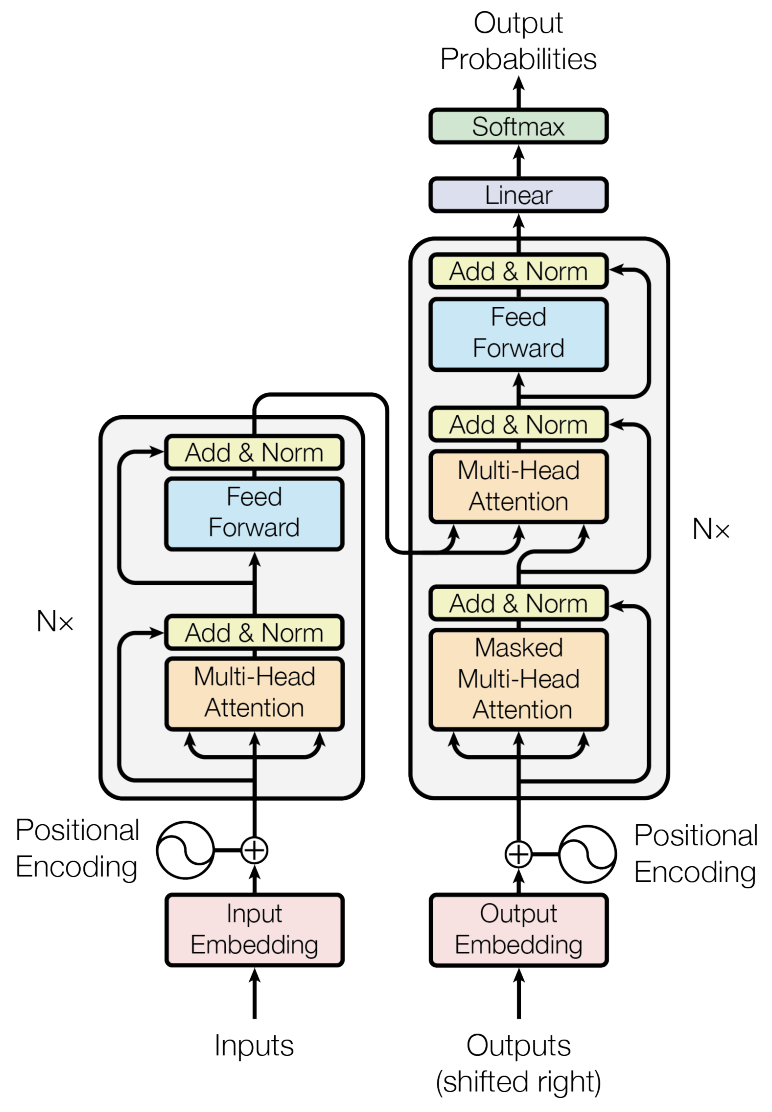
\includegraphics[scale=0.8]{figuras/intro-bert-transformers.png}
    % \caption[Así aparece el rótulo en el índice]{Así aparece el rótulo en el texto.}
    \caption[BERT - Arquitectura de Transformer]{\textbf{Arquitectura del modelo Transformer propuesto en el \textit{paper} ``Attention is all you need!''. Fuente: \citep{https://doi.org/10.48550/arxiv.1706.03762}}}
    \label{fig-intro-bert-transformers}
\end{figure}

La publicación del \textit{paper} \textit{``Attention is all you need''} \citep{https://doi.org/10.48550/arxiv.1706.03762} representó una completa revolución en el campo del procesamiento del lenguaje natural. En este \textit{paper} se propone por primera vez la arquitectura \Gls{gls_transformer} (figura \ref{fig-intro-bert-transformers}). La clave de esta novedosa arquitectura es el mecanismo de autoatención y el uso de autoencoders para lograr un entrenamiento más ágil y producir resultados eficientes. En la actualidad, años después de la publicación del \textit{paper}, esta arquitectura sigue siendo estado del arte en el mundo del NLP y la base de implementaciones como BERT o GPT.

Aunque las \acrshort{acr_rnn}s permiten observar palabras anteriores de la secuencia, sufren de memoria cortoplacista. Esto provoca que cuando trabajamos con una secuencia larga las \acrshort{acr_rnn}s no pueden observar palabras muy antiguas. Las \acrshort{acr_lstm}s tienen una ventana de memoria más grande que las \acrshort{acr_rnn}s, pero siguen teniendo una capacidad limitada. Esta secuencialidad es un obstáculo para la paralelización del proceso. Además, cuando estas secuencias son demasiado largas, el modelo tiende a olvidar el contenido de las posiciones distantes en la secuencia o a mezclarlo con el contenido de las posiciones siguientes. El mecanismo de autoatención resuelve esto ya que, permiten modelar dependencias sin considerar su distancia en las secuencias de entrada o salida. En la mayoría de los casos los mecanismos de atención se utilizan en conjunto con una red recurrente.

El Transformer utiliza dos tipos diferentes de funciones de atención (figura \ref{fig-intro-bert-attention}):
\begin{itemize}
    \item \textbf{Atención de producto punto escalado} o \textit{scaled dot-product attention}, que calcula la función de atención en un conjunto de consultas simultáneamente, empaquetadas en una matriz. 
    \item \textbf{Atención Multi-Cabeza} o \textit{Multi-Head Attention}, que permite que el modelo atienda de manera conjunta la información de diferentes subespacios de representación en diferentes posiciones.
\end{itemize}

\begin{figure}[ht!]
    \centering
    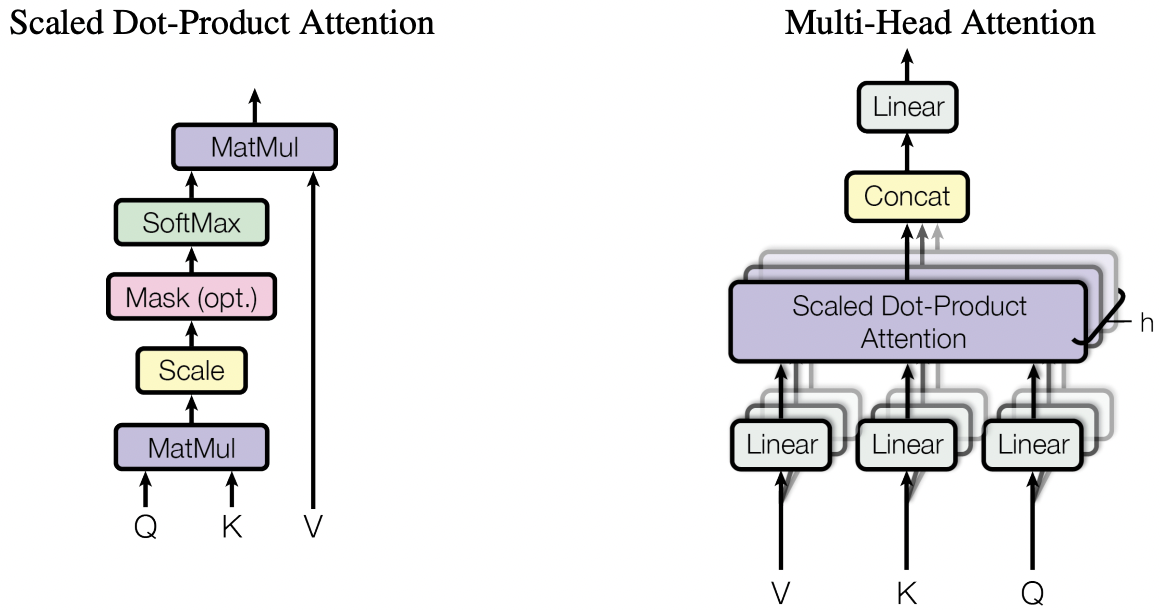
\includegraphics[scale=0.7]{figuras/intro-bert-attention.png}
    % \caption[Así aparece el rótulo en el índice]{Así aparece el rótulo en el texto.}
    \caption[BERT - Mecanismos de Atención]{\textbf{A la izquierda podemos observar el mecanismo de atención basado en el producto punto escalado y a la derecha el mecanismo de atención multi-head, el cual consiste en varias capaz de atención corriendo en paralelo. Fuente: \citep{https://doi.org/10.48550/arxiv.1706.03762}}}
    \label{fig-intro-bert-attention}
\end{figure}

En cuanto a las entradas, el \textit{paper} de \cite{https://doi.org/10.48550/arxiv.1706.03762} menciona que las secuencias de entrada se representan utilizando alguna forma de \gls{gls_wordembeddings}, es decir, una representación vectorial de cada palabra que guarda información semántica. Esto se hace tanto para el \textit{encoder} como para el \textit{decoder}. Los \gls{gls_wordembeddings} por sí solos carecen de cualquier información posicional que se logra en las \acrshort{acr_rnn}s en virtud de su naturaleza secuencial. Mientras tanto, en la autoatención se pierde cualquier información posicional debido a la aplicación de la función \gls{gls_softmax}. Para preservar la información posicional, el \Gls{gls_transformer} inyecta un vector a los embeddings de entrada individuales. Este vector inyectado se denomina ``codificación posicional'' y se agrega a los \textit{embeddings} de entrada en la parte inferior de las pilas del \textit{encoder} y \textit{decoder}.

Los autores compararon los resultados de la arquitectura con otras soluciones consideradas estado del arte en 2017. La arquitectura \Gls{gls_transformer} obtuvo un desempeño mejor que el de otros modelos. (figura \ref{fig-intro-bert-transresults}) 

\begin{figure}[ht!]
    \centering
    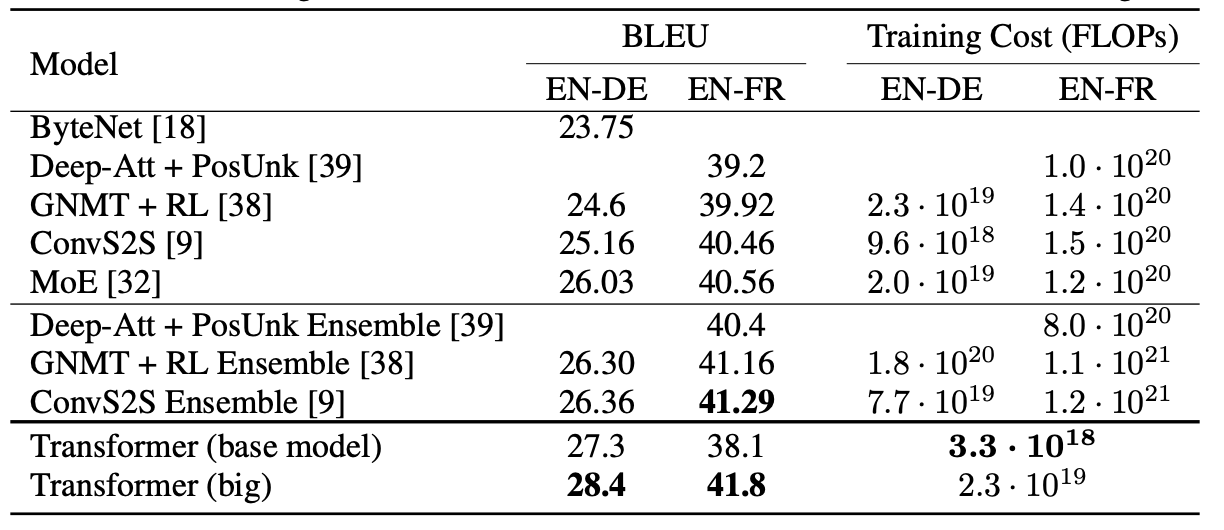
\includegraphics[scale=0.6]{figuras/intro-bert-transresults.png}
    % \caption[Así aparece el rótulo en el índice]{Así aparece el rótulo en el texto.}
    \caption[BERT - Transformer Resultados]{\textbf{La imagen compara el resultado de la implementación de la arquitectura \Gls{gls_transformer} en un problema de traducción superando el desempeño de otros modelos considerados el estado del arte antes de la publicación del \textit{paper} ``All you Need is Attention''. En la comparación se observa además de un mejor desempeño, un costo de procesamiento menor al del resto de modelos. Fuente: \cite{https://doi.org/10.48550/arxiv.1706.03762}}}
    \label{fig-intro-bert-transresults}
\end{figure}

\subsection{Arquitectura de BERT}
\label{subsection-arquitectura-bert}

La arquitectura de BERT es básicamente una pila de \textit{encoders} de la arquitectura \Gls{gls_transformer}. 

En el \textit{paper} original de BERT \cite{https://doi.org/10.48550/arxiv.1810.04805} hablan de dos modelos o versiones de BERT que se pueden elegir en términos de implementación:

\begin{itemize}
    \item \textbf{BERT$_{BASE}$:} L=12, H=768, A=12, 110 millones de parámetros.
    \item \textbf{BERT$_{LARGE}$:} L=24, H=1024, A=16, 340 millones de parámetros.
\end{itemize}

donde:\\
L: número de capas de encoders\\
H: tamaño de la capa oculta (dimensión del embedding)\\
A: número de encabezados de auto atención\\

La innovación técnica clave de BERT es aplicar el entrenamiento bidireccional de \Gls{gls_transformer} al modelamiento del lenguaje. Esto es diferente a los enfoques de modelos anteriores que analizaban las secuencias de texto en una sola dirección. Los resultados obtenidos por \cite{https://doi.org/10.48550/arxiv.1810.04805} en su \textit{paper}, muestran que un modelo de lenguaje entrenado bidireccionalmente tiene un sentido más profundo del contexto y flujo del lenguaje que los modelos de lenguaje de una sola dirección. 

El preentrenamiento de BERT está basado en dos tareas no supervisadas:

\begin{enumerate}
    \item \textbf{Modelo de Lenguaje Enmascarado} o \textit{Masked Language Model} (MLM): esta tarea es la que habilita el aprendizaje bidereccional profundo en el modelo. En esta tarea se enmascara un porcentaje de los tokens de entrada (reemplazando los tokens por el token especial [MASK]) al azar y el modelo intenta predecir los tokens que han sido enmascarados. Esos tokens predichos del modelo luego son introducidos a una función softmax de salida sobre el vocabulario para obtener las palabras de salida finales.
    \item  \textbf{Predicción de la Siguiente Oración} o \textit{Next Sentence Prediction} (NSP): esta tarea es la utilizada para que el modelo sea capaz de resolver tareas donde es importante la relación entre dos oraciones. En este caso, el modelo es entrenado recibiendo pares de frases como entrada y aprendiendo a predecir si la segunda frase del par es la subsiguiente dentro del documento original de entrada.
\end{enumerate}

El modelo esta entrenado en ambas tareas mencionadas anteriormente de forma simultánea. Esto es posible debido a la forma en la que el modelo procesa las entradas y las salidas, las cuales son compatibles para ambos problemas. 

En cuanto a la entrada (ver figura \ref{fig-intro-bert-transresults}), BERT necesita recibir información tanto para una sola oración como para dos oraciones agrupadas sin ambigüedades en una secuencia de token. Los autores del \textit{paper} oficial señalan que una secuencia de entrada puede ser un tramo arbitrario de texto contiguo, en lugar de una oración lingüística real. El token [SEP] se usa para separar dos oraciones.

A diferencia de las \acrshort{acr_rnn}s en las que las entradas se alimentan secuencialmente, el modelo BERT no puede conservar el orden de los tokens de entrada. El orden de las palabras en cada idioma es significativo, tanto semántica como sintácticamente. Para realizar correctamente la tarea de predicción de la siguiente oración, el modelo debe ser capaz de distinguir entre las dos oraciones. Ambos problemas se resuelven agregando \textit{embeddings} que contienen la información requerida a los tokens correspondientes a la entrada original y usando el resultado como entrada a nuestro modelo BERT. 

\begin{figure}[ht!]
    \centering
    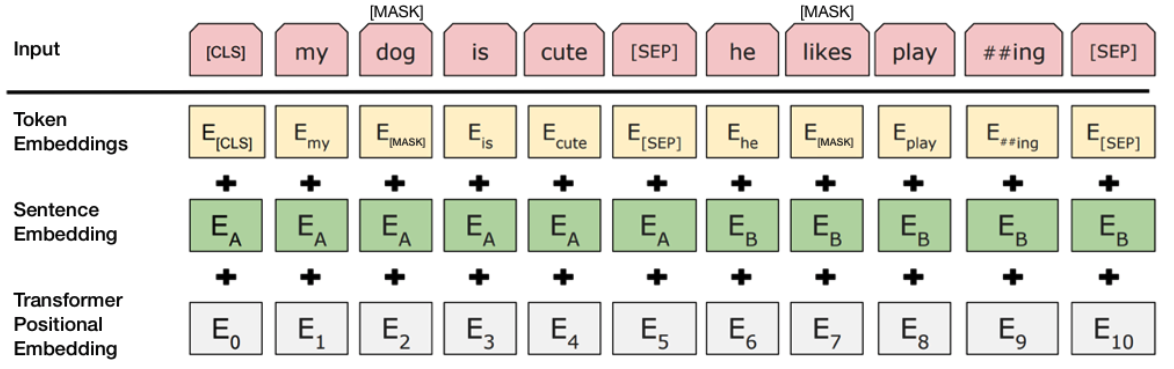
\includegraphics[scale=0.3]{figuras/intro-bert-tokens.png}
    % \caption[Así aparece el rótulo en el índice]{Así aparece el rótulo en el texto.}
    \caption[BERT - Token Embeddings]{\textbf{Representación de la entrada del modelo de BERT. El input del modelo es la suma de los token embeddings, el embedding de segmentación y el embedding posicional. Fuente: \cite{https://doi.org/10.48550/arxiv.1706.03762}}}
    \label{fig-intro-bert-tokens}
\end{figure}

Los siguientes \textit{embeddings} se agregan a los \textit{embeddings} de tokens:

\begin{itemize}
    \item \textbf{Embedding de segmentos} o \textit{Segment Embedding}: Proporciona información sobre la oración de la que forma parte un token en particular.
    \item  \textbf{Embedding posicional} o \textit{Position Embedding}: Proporciona información sobre el orden de las palabras de entrada.
\end{itemize}

En cuanto a la salida, también está diseñada para predecir el resultado de dos tareas diferentes de forma simultánea. Esto lo hace mediante el uso de diferentes capas \acrshort{acr_ffnn} y \gls{gls_softmax} construidas sobre las salidas del último \textit{encoder}. El primer token de entrada es siempre un token de clasificación especial [CLS]. El estado final correspondiente a este token se usa como la representación de secuencia agregada para las tareas de clasificación y se usa para la predicción de la siguiente oración. Los estados finales correspondientes a los tokens [MASK] se introducen en la \acrshort{acr_ffnn} y \gls{gls_softmax} para predecir la siguiente palabra del vocabulario.

\subsection{BERT y Fine Tunning}
\label{subsection-bert-finetunning}

La idea de la transferencia de aprendizaje o \textit{transfer learning} (en inglés), es entrenar un modelo en una tarea y luego aprovechar el conocimiento adquirido para mejorar el rendimiento del modelo en una tarea relacionada. El \textit{fine-tunning} es un enfoque para transferir el aprendizaje en el que se agrega una capa a la salida del modelo para que se ajuste a una nueva tarea y se entrena el modelo resultante.

Una consecuencia positiva de agregar capas (entrada/salida) y no cambiar el modelo BERT es que solo se necesita aprender una cantidad mínima de parámetros desde cero, lo que hace que el procedimiento sea rápido, rentable y eficiente en recursos.

En la clasificación de pares de oraciones y la clasificación de oraciones únicas, el estado final correspondiente al token [CLS] se usa como entrada para las capas adicionales que hacen la predicción. (ver figura \ref{fig-intro-bert-finetunning})

\begin{figure}[ht!]
    \centering
    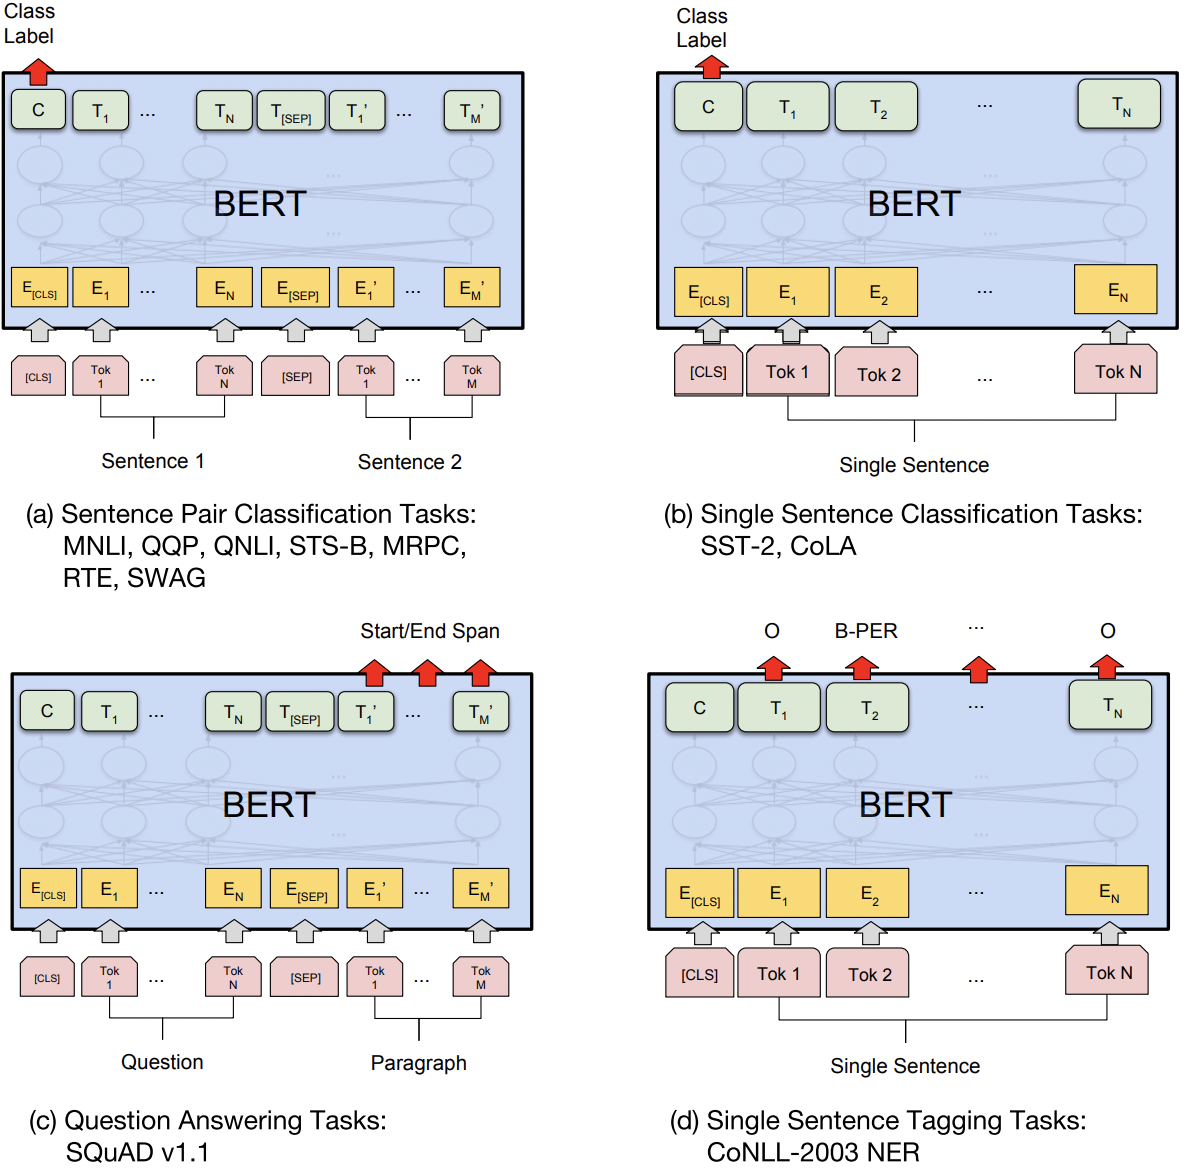
\includegraphics[scale=0.6]{figuras/intro-bert-finetunning.png}
    % \caption[Así aparece el rótulo en el índice]{Así aparece el rótulo en el texto.}
    \caption[BERT - Fine-tunning]{\textbf{Esta imagen ilustra el proceso de fine-tunning para BERT en diferentes tareas y como se amolda la arquitectura unificada para distintas tareas. Fuente: \cite{https://doi.org/10.48550/arxiv.1706.03762}}}
    \label{fig-intro-bert-finetunning}
\end{figure}

En las tareas de preguntas y respuestas, se introducen un vector de inicio (S) y uno final (E) durante el \textit{fine-tunning}. La pregunta se introduce al modelo como oración A y la respuesta como oración B. La probabilidad de que la palabra i sea el comienzo del intervalo de respuesta se calcula como un producto escalar entre Ti (estado final correspondiente al i-ésimo token de entrada) y S (vector de inicio) seguido por un \textit{softmax} sobre todas las palabras del párrafo. Se utiliza un método similar para el tramo final. (ver figura \ref{fig-intro-bert-finetunning})

Entre las ventajas del proceso de \textit{fine-tunning} podemos mencionar:

\begin{itemize}
    \item \textbf{Desarrollo más rápido}
En primer lugar, los pesos del modelo BERT preentrenados ya codifican mucha información sobre el lenguaje. Como resultado, lleva mucho menos tiempo entrenar el modelo ajustado, es como si ya se hubiera entrenado las capas inferiores de nuestra red de forma exhaustiva y solo se necesita ajustar levemente mientras se usa su salida como características para la tarea de clasificación. De hecho, los autores recomiendan solo de 2 a 4 épocas de entrenamiento para ajustar BERT en una tarea específica de NLP, en comparación con los cientos de horas de \acrlong{acr_gpu} (\acrshort{acr_gpu}, por sus siglas en inglés) necesarias para entrenar el modelo BERT original o una LSTM desde cero.
\item \textbf{Menos datos}
Además, y quizás igual de importante, debido a los pesos previamente entrenados, este método permite ajustar una tarea en un conjunto de datos mucho más pequeño que el que se requeriría en un modelo construido desde cero. Un inconveniente importante de los modelos NLP creados \textit{from scratch} es que a menudo se requiere de un conjunto de datos prohibitivamente grande para entrenar nuestra red con una precisión razonable, lo que significa que se tiene que dedicar mucho tiempo y energía a la creación del conjunto de datos. Al ajustar BERT, ahora se puede entrenar un modelo para que tenga un buen rendimiento con una cantidad mucho menor de datos de entrenamiento.
\item \textbf{Mejores resultados}
Finalmente, se demostró que este sencillo procedimiento de ajuste fino (por lo general, agregar una capa completamente conectada encima de BERT y entrenar durante algunas épocas) logra resultados de vanguardia con ajustes mínimos específicos de tareas para una amplia variedad de tareas: clasificación, inferencia de lenguaje, similitud semántica, respuesta a preguntas, etc. En lugar de implementar arquitecturas personalizadas, se ha demostrado que funciona bien en una tarea específica, simplemente ajustar BERT. Esta opción se muestra como una alternativa mejor (o al menos igual).
\end{itemize}

\subsection{BERT, variantes y otros modelos}
\label{subsection-bert-otros}

BERT no es el único modelo que está produciendo estos resultados innovadores. Existe otro modelo desarrollado por OpenAI llamado GPT-3 \citep{articleBrownGPT3} que está causando bastante revuelo en el mundo del NLP.  

GPT ha causado bastante revuelo en Internet últimamente. Este modelo tiene algo en común con BERT, y es que ambos modelos reutilizan un componente de \Gls{gls_transformer}. Como se indicó anteriormente, BERT apila la parte del encoder del \Gls{gls_transformer} como su bloque de construcción. Mientras tanto, GPT usa la parte del decoder del \Gls{gls_transformer} como su bloque de construcción.

Las conexiones bidireccionales en BERT se deben a la autoatención bidireccional del \textit{encoder}. Mientras tanto, las conexiones en GPT solo están en una sola dirección, de izquierda a derecha, debido al diseño del \textit{decoder} para evitar mirar predicciones futuras.

Adicionalmente, hay algunas variantes de BERT donde la arquitectura no es diferente, pero presentan ciertas adecuaciones. (ver tabla \ref{tbl-bert-variants}) 

Paste Latex Here\begin{table}[ht!]
\resizebox{\textwidth}{!}{
	\begin{tabular}{l|c|p{9cm}}
		\toprule
		\textbf{Modelo}                                                         & \textbf{Creador} & \textbf{Descripción}                                                                                                                                                                                                                                                                                                                          \\ \midrule
		Albert \cite{ALBERT_https://doi.org/10.48550/arxiv.1909.11942}          & Google           & Este paper describe técnicas de reducción de parámetros para disminuir la reducción de memoria y aumentar la velocidad de entrenamiento de los modelos BERT.                                                                                                                                                                               \\ \midrule
		RoBERTa \cite{ROBERTA_https://doi.org/10.48550/arxiv.1907.11692}        & Facebook         & Este paper cree que los modelos BERT originales estaban poco entrenados y muestra que con más entrenamiento/ajuste puede superar los resultados iniciales.                                                                                                                                                                                    \\ \midrule
		ERNIE \cite{ERNIE_https://doi.org/10.48550/arxiv.1904.09223}            & -                & Representación mejorada a través de la integración del conocimiento de Baidu: se inspira en la estrategia de enmascaramiento de BERT y aprende la representación del lenguaje mejorada mediante estrategias de enmascaramiento del conocimiento, que incluyen el enmascaramiento a nivel de entidad y el enmascaramiento a nivel de frase. \\ \midrule
		DistilBERT  \cite{DISTILBERT_https://doi.org/10.48550/arxiv.1910.01108} & -                & BERT más pequeño. Reduce el número de capas a 6 y elimina el embedding de segmentación                                                                                                                                                                                                                                                     \\ \bottomrule
	\end{tabular}
}
% \caption[Así aparece el rótulo en el índice]{Así aparece el rótulo en el texto.}
\caption[BERT - Otros modelos de lenguaje basados en BERT]{\textbf{Lista de modelos basados en BERT. Fuente: \cite{articleBrownGPT3}}}
\label{tbl-bert-variants}
\end{table}